\section{Design of the LNA}

\subsection{Transistor Bias Network}

The DC bias point of a transistor directly influences its small-signal S-parameters, and hence the gain, noise figure and stability of the LNA. This makes this step crucial.
Figure \ref{fig:DCBiasNPN} shows the biasing circuit and its Thévenin equivalent used to simplify analysis.

\begin{figure}[H]
    \centering
    \begin{subfigure}{0.4\textwidth}
        \includegraphics*[scale = 0.3]{Images/DCBiasNPN.png}
        \caption{Transistor DC biasing circuit}
    \end{subfigure}
    \hfill
    \begin{subfigure}{0.4\textwidth}
        \includegraphics*[scale = 0.3]{Images/VthBiasCircuit.png}
        \caption{Bias circuit equivalent circuit}
        \label{fig:DCBiasTh}
    \end{subfigure}
    \label{fig:DCBiasNPN}
\end{figure}

As shown in Figure \ref{fig:DCBiasTh} the Thévenin equivalent is given by the equations \ref{eq:biasThev}, replacing the $R_1$, $R_2$ voltage divider.

\begin{equation}
    \begin{split}
        R_{TH} &= R_1//R_2\\
        V_{TH} &= V_{cc}\frac{R_2}{R_1+R_2}
    \end{split}
    \label{eq:biasThev}
\end{equation}

Using Kirchhoff voltage law, the equations \ref{eq:biasKVL} are derived, the first starts at $V_{TH}$ goes through $R_{TH}$, $V_{BE}$ and $R_4$. The second goes from $V_{CC}$ through $R_3$, $V_{CE}$ and $R_4$. 

\begin{equation}
    \begin{cases}        
        0 = V_{TH} -I_b\cdot R_{TH} - V_{BE}-I_E\cdot R_4  \\
        0 = V_{CC} - R_3\cdot I_C - V_{CE} - I_E \cdot R_4\\
    \end{cases}
    \label{eq:biasKVL}
\end{equation}

Solving the system of equations, assuming fixed values for $R_2$ and $R_4$, originates the equations \ref{eq:biasr1r3}.

\begin{equation}
    \begin{split}
        R_1 &= \frac{R_{2} \left(- I_{C} R_{4} \beta - I_{C} R_{4} - V_{BE} \beta + V_ {CC} \beta\right)}{I_{C} R_{2} + I_{C} R_{4} \beta + I_{C} R_{4} + V_{BE} \beta}\\
        R_3 &= \frac{- I_{C} R_{4} \beta - I_{C} R_{4} + V_{CC} \beta - V_{CE} \beta}{I_{C} \beta}
    \end{split}
    \label{eq:biasr1r3}
\end{equation}

The Table \ref{tab:BiasParam}, shows the provided values for the biasing circuit and the fixed values for $R_2$ and $R_4$.

\begin{table}[h]
    \centering
    \caption{Transistor biasing parameters}
    \begin{tabularx}{\textwidth}{>{\centering\arraybackslash}X >{\centering\arraybackslash}X >{\centering\arraybackslash}X >{\centering\arraybackslash}X}
        \toprule
        \textbf{Parameter} & \textbf{Value} \\
        \midrule
        $R_2$     & $1\,\si{\kilo\ohm}$ \\
        \midrule
        $R_4$     & $100\,\si{\ohm}$\\
        \midrule
        $\beta$   & $72.534$ \\
        \midrule
        $I_C$     & $9\,\si{\milli\ampere}$ \\
        \midrule
        $V_{CC}$  & $10\,\si{\volt}$ \\
        \midrule
        $V_{BE}$  & $1\,\si{\volt}$ \\
        \midrule
        $V_{CE}$  & $\SI{5}{\volt}$\\
        \bottomrule
    \end{tabularx}
    \label{tab:BiasParam}
\end{table}

Resulting in $R_1 = \SI{4}{\kilo\ohm}$ and $R_3 = \SI{454}{\ohm}$.

%\textcolor{red}{FALTA SIM E JUSTIFICAR A SIM}

\subsection{S-parameters with packaging effects}

With the biasing circuit designed, the next step was to simulate the S-parameters of the transistor in LTSpice.  The S-parameters were taken for a frequency range of $1\,\si{\giga\hertz}$ to $10\,\si{\giga\hertz}$, Figure \ref{fig:withoutmathing} shows the S-parameters of the transistor without any matching network.

\begin{figure}[H]
    \centering
    \includegraphics[width=0.8\textwidth]{Images/without-matching.png}
    \caption{S-parameters of the transistor without matching network}
    \label{fig:withoutmathing}
\end{figure}

%\subsection{Transistor validation for the given bias point}

% The transistor standstill operating point was simulated in LTSpice, and the results are shown in Figure \ref{fig:op-bias}. 

% \begin{figure}[H]
%     \centering
%     \includegraphics[width=0.8\textwidth]{Images/OpBias.png}
%     \caption{Transistor operating point}
%     \label{fig:op-bias}
% \end{figure}
\subsection{Stability}


Ensuring that the LNA remains stable is critical for reliable operation. The network is unconditionally stable for a frequency if for any source impedance value, $|\rho_{in}|<1$  and for the load impedance $|\rho_{out}|<1$.
The stability circles can be used to determine regions for $\rho_{in}$ and $\rho_{out}$ where the amplifier circuit will be conditionally stable, but simpler tests can be used to determine unconditional stability. 


Defining $K$ as:

\begin{equation}
    K = \frac{1-|S_{11}|^2-|S_{22}|^2+|\Delta|^2}{2|S_{12}\cdot S_{21}|}
\end{equation}

If:
\begin{itemize}
    \item $K>1$ and $|\Delta|<1\rightarrow$ unconditionally stable
    \item $K>1$ and $|\Delta| > 1$ or  $K<1 \rightarrow$ potentially unstable or always unstable
\end{itemize}

Another criteria is the $\mu$ factor,

Defining $\mu$ as:
$$\mu = \frac{1-|S_{11}|^2}{|S_{22}-\Delta S_{11}^*| + |S_{12}\cdot S_{21}|}$$

if $\mu > 1\rightarrow$ unconditionally stable
In addition, it can be said that larger values of $\mu$ imply greater stability.

\begin{figure}[H]
    \centering
    \includegraphics*[scale = 0.5]{Images/KFactor.png}
    \caption{Stability tests}
    \label{fig:StabilityTest}
\end{figure}

Figure \ref{fig:StabilityTest}, shows that the LNA is stable for frequencies above $\SI{3.1}{\giga\hertz}$ and above $\SI{10}{\giga\hertz}$ loses stability again.

At this stage another important figure is the Maximum Available Gain, $MAG$, which for the bilateral case can be expressed as the equation \ref{eq:MAG}.

\begin{equation}
    MAG = \left | \frac{S_{21}}{S_{12}} \right |\cdot \left[ K \pm \sqrt{K^2-1} \right]
    \label{eq:MAG}
\end{equation}

\begin{figure}[H]
    \centering
    \includegraphics*[scale = 0.5]{Images/MAG.png}
    \caption{Maximum Available Gain }
    \label{fig:MAG}
\end{figure}

Now having the full picture of the LNA characteristics, an operating frequency can be decided. It is a compromise between stability and gain. The frequency chosen was $\SI{4}{\giga\hertz}$.


\subsection{Input and output matching networks for maximum gain}

The adaptation for maximum gain is done using the line impedance transformation method. The input and output matching networks are designed to transform the input and output impedances of the transistor to the desired values, which are $50\,\si{\ohm}$ in this case. In the Smith chat, the matching is done with inductors and capacitors and lines and stubs.

\subsubsection{Matching with lumped elements}

The matching networks are designed using the Smith chart, which allows for the visualization of the impedance transformation. The input and output impedances of the transistor are transformed to $50\,\si{\ohm}$ using a combination of inductors and capacitors. The values of the components are also calculated using the equations for impedance transformation.

The matching using the Smith Chart for the input and output are shown in Figures \ref{fig:zs-LC-matching} and \ref{fig:zl-LC-matching}, where the input and output impedances of the transistor are transformed to $50\,\si{\ohm}$ using a combination of inductors and capacitors.

\begin{figure}[H]
    \centering
    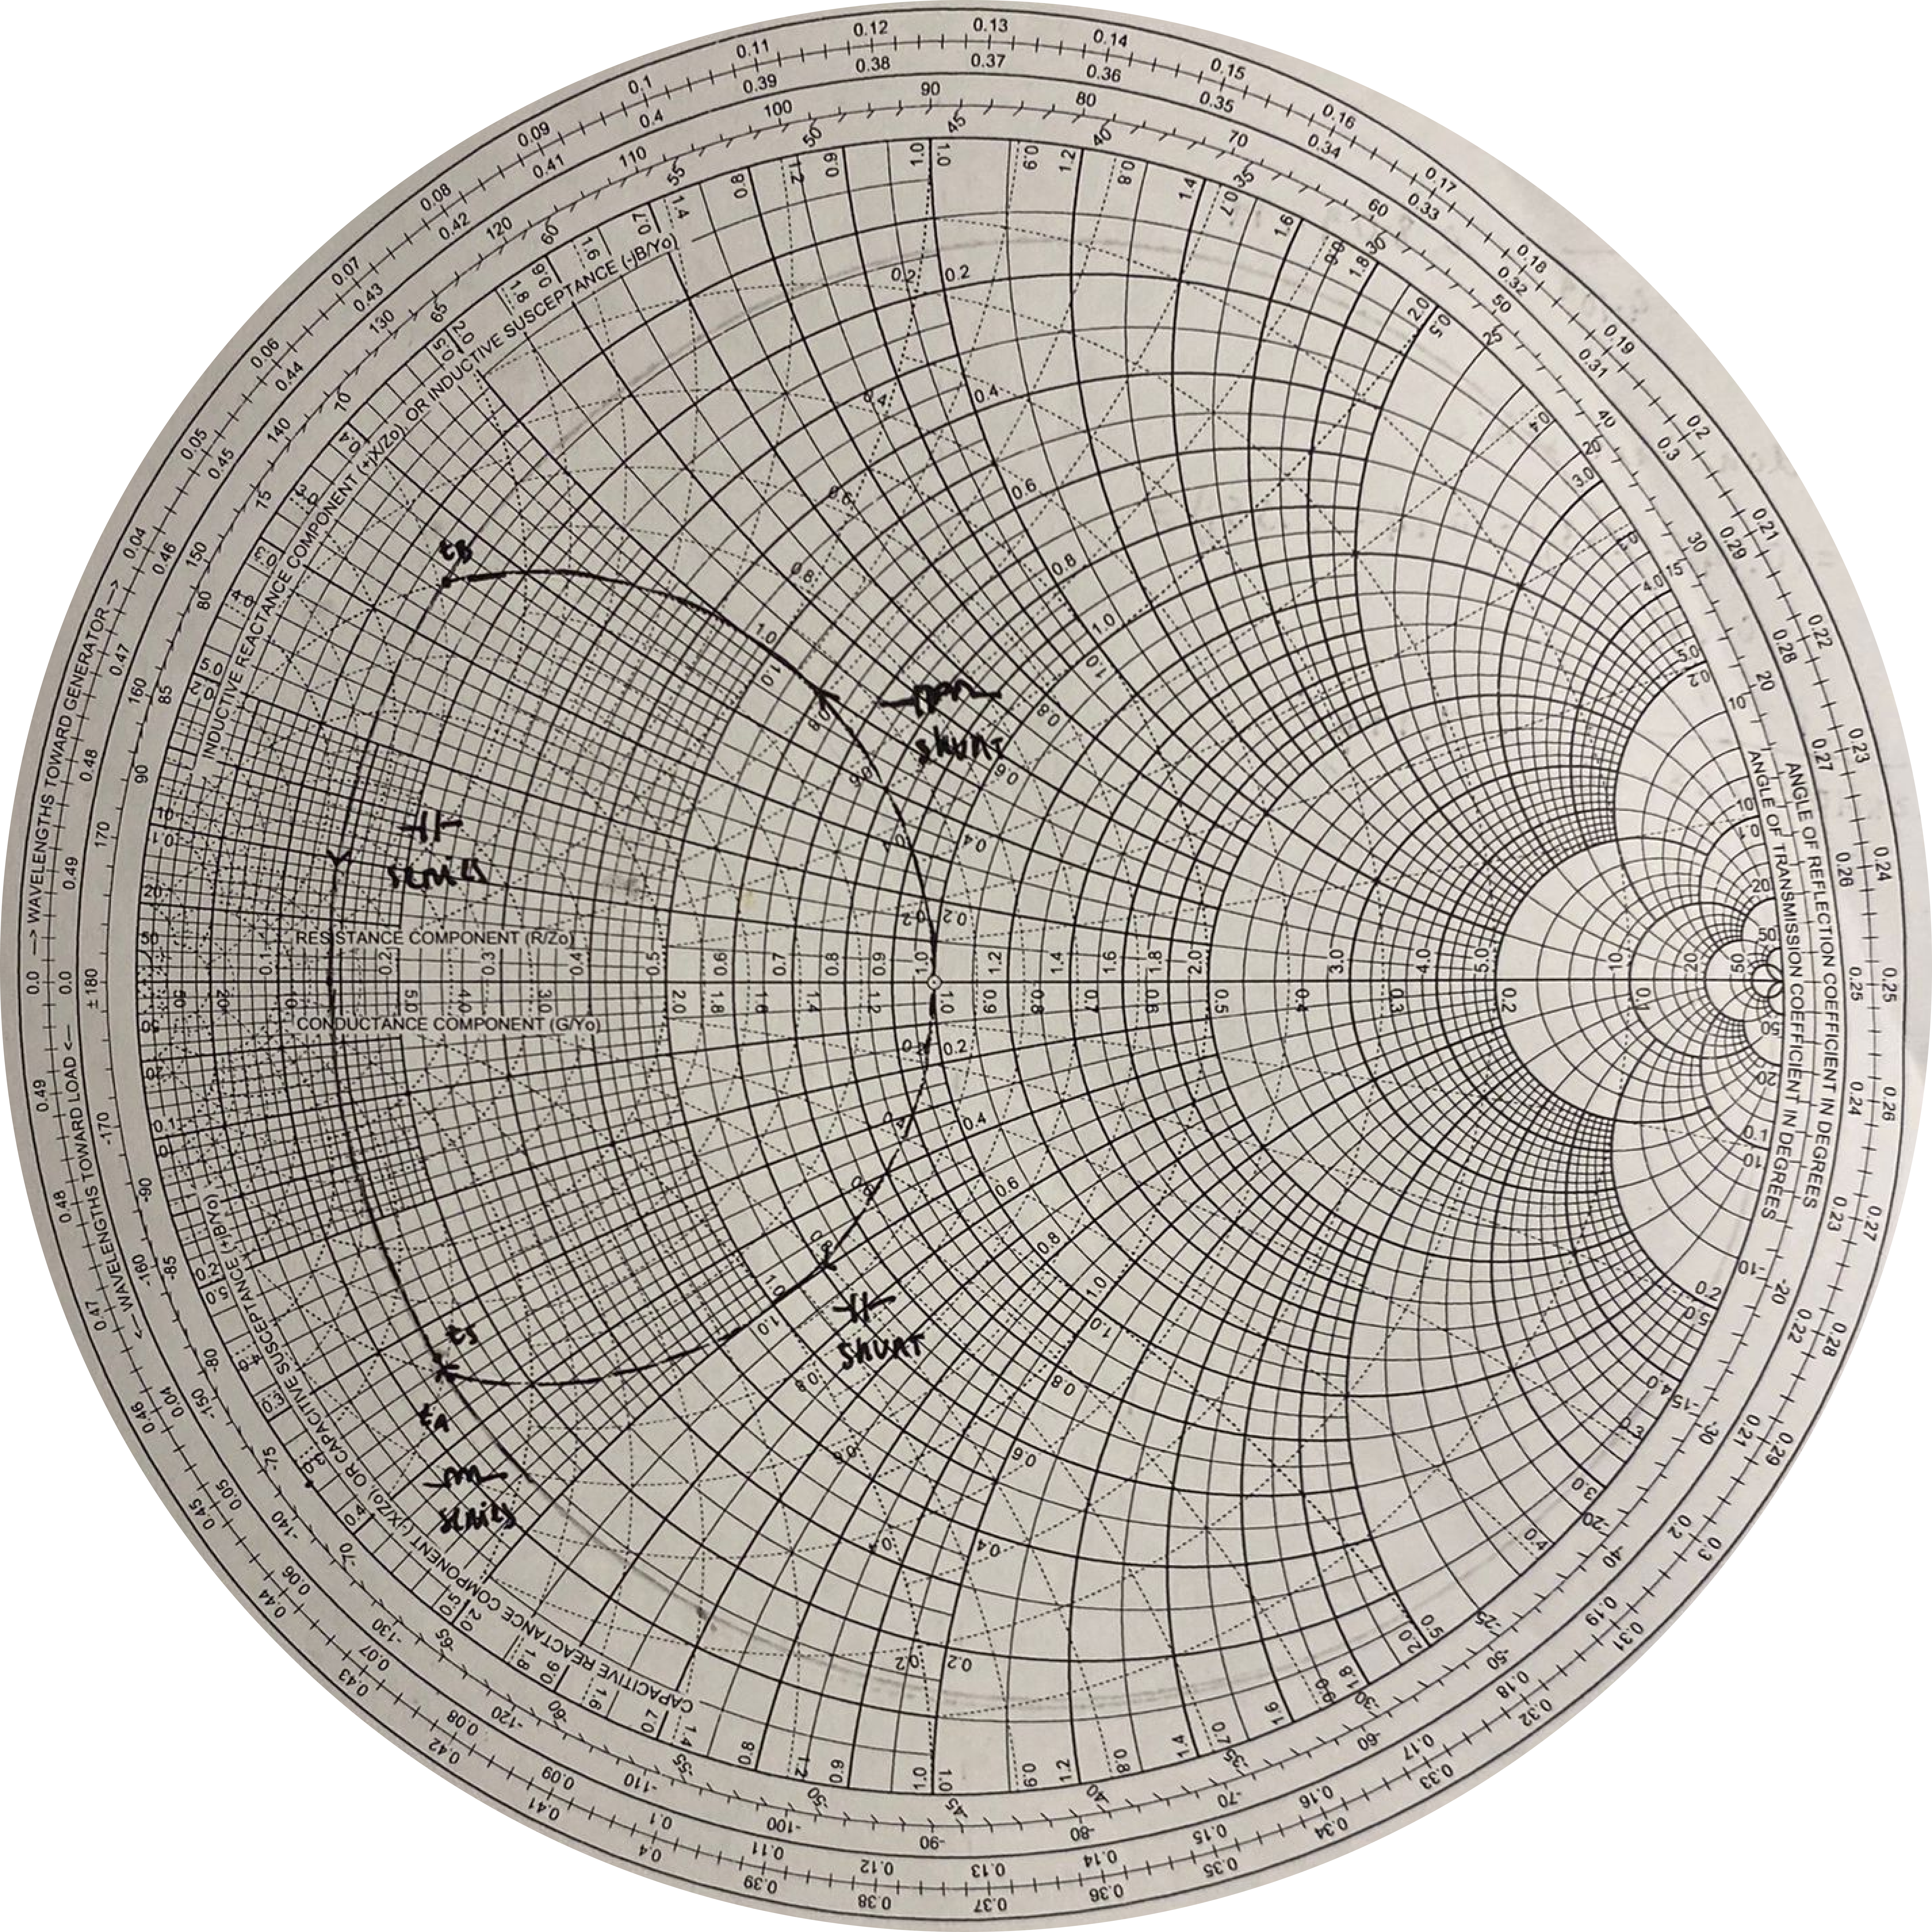
\includegraphics[width=0.5\textwidth]{Images/zs-LC-matching.png}
    \caption{Smith chart for input matching with lumped elements}
    \label{fig:zs-LC-matching}
\end{figure}

The adaptation mesh for the input was done with a shunt inductor and a series capacitor and the equivalent circuit is shown in Figure \ref{fig:MatchingCircuit-input}. The values of the components were also calculated using the equations for impedance transformation as a form of validation.

\begin{figure}[H]
    \centering
    \includegraphics[width=0.5\textwidth]{Images/Input-matching-circuit.png}
    \caption{Matching circuit for input}
    \label{fig:MatchingCircuit-input}
\end{figure}

\begin{figure}[H]
    \centering
    \includegraphics[width=0.5\textwidth]{Images/zl-LC-matching.png}
    \caption{Smith chart for output matching with lumped elements}
    \label{fig:zl-LC-matching}
\end{figure}

The adaptation mesh for the output is done with a series capacitor and a shunt inductor and the equivalent circuit is shown in Figure \ref{fig:MatchingCircuit-output}. The values of the components were also calculated using the equations for impedance transformation as a form of validation.

\begin{figure}[H]
    \centering
    \includegraphics[width=0.5\textwidth]{Images/Ouput-matching-circuit.png}
    \caption{Matching circuit for output}
    \label{fig:MatchingCircuit-output} 
\end{figure}

The resulting circuit is shown in Figure \ref{fig:MatchingCircuit}, where the input and output matching networks are designed using a combination of inductors and capacitors.

\begin{figure}[H]
    \centering
    \includegraphics[width=0.8\textwidth]{Images/LC_matching-circuit.png}
    \caption{Matching circuit for input and output with values}
    \label{fig:MatchingCircuit}
\end{figure}

\subsubsection{Matching lines and stubs}
The matching networks were also designed using transmission lines and stubs, this type of adaptation allows grater frequencies (more than 1 \si{\giga \hertz}) in real conditions. The input and output impedances of the transistor are transformed to $50\,\si{\ohm}$ using a combination of transmission lines and stubs. The values of the components are also calculated using the equations for impedance transformation to validate the results.

The matching using the Smith Chart for the input and output are shown in Figures \ref{fig:zs-line-matching} and \ref{fig:zl-line-matching}.

\begin{figure}[H]
    \centering
    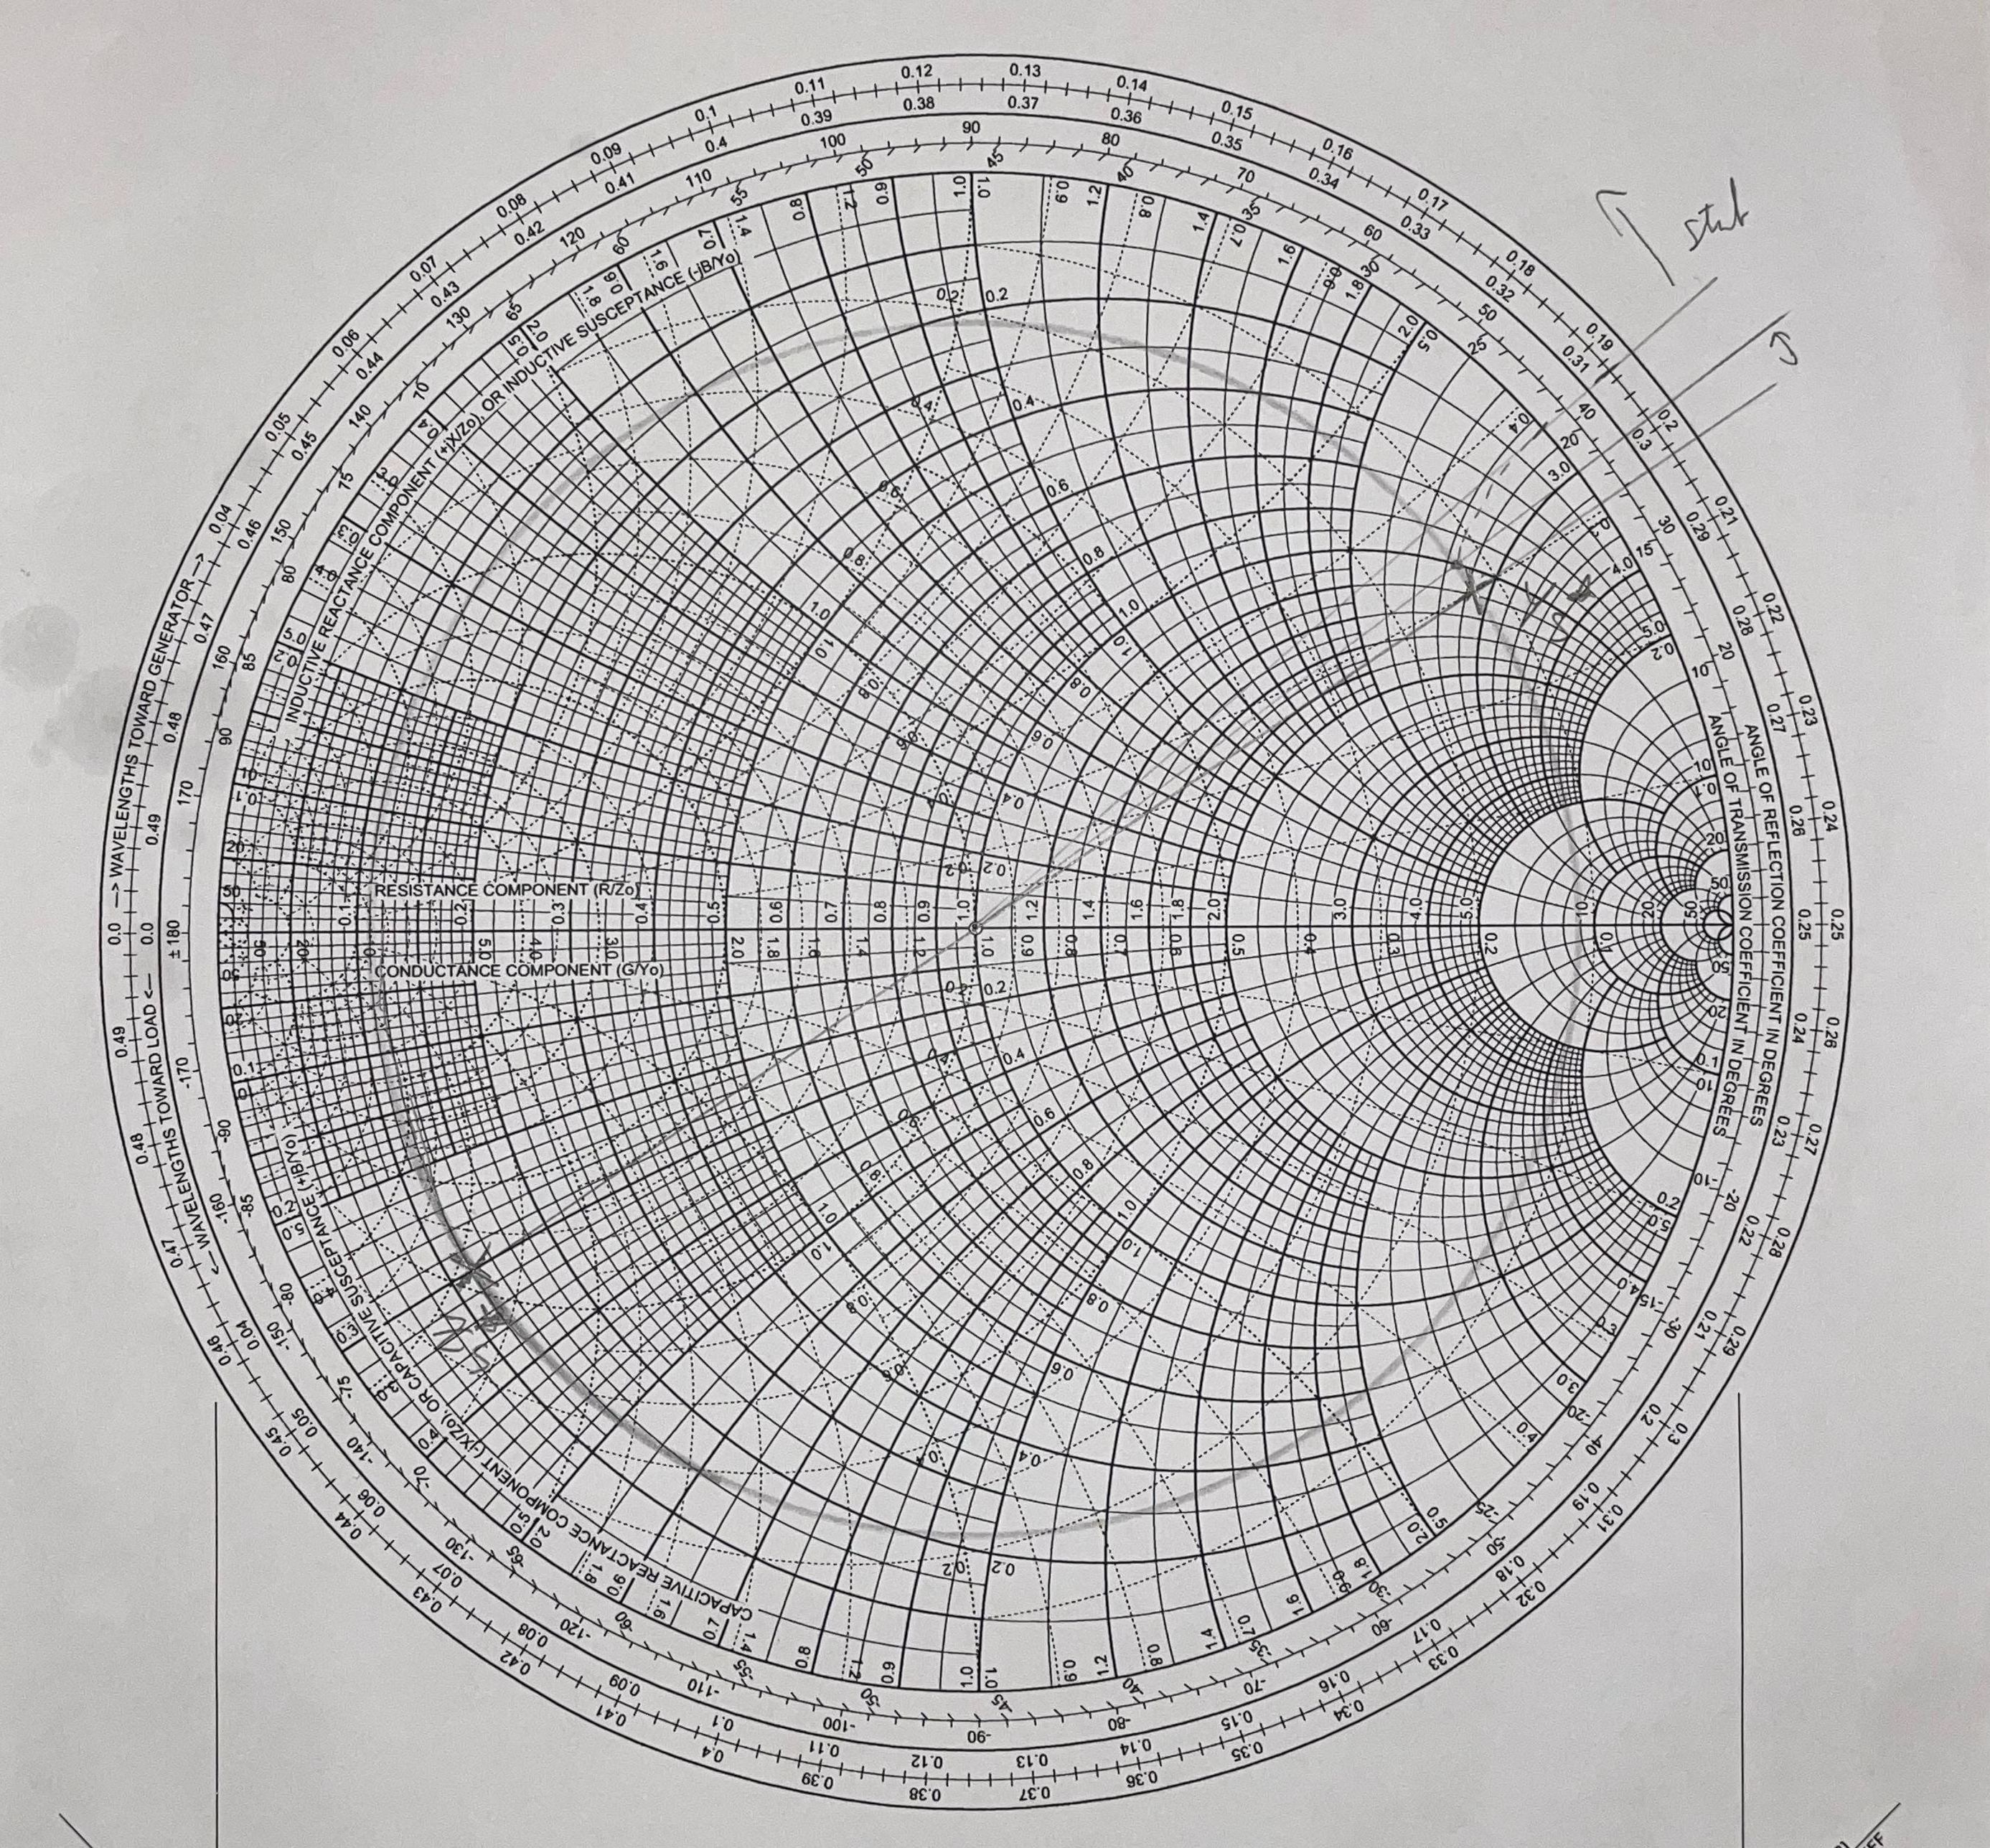
\includegraphics[width=0.5\textwidth]{Images/zs-LS-matching.png}
    \caption{Smith chart for input matching with lines and stubs}
    \label{fig:zs-line-matching}
\end{figure}

The adaptation mesh for the input was done with an open circuit shunt stub and a series line. 

\begin{figure}[H]
    \centering
    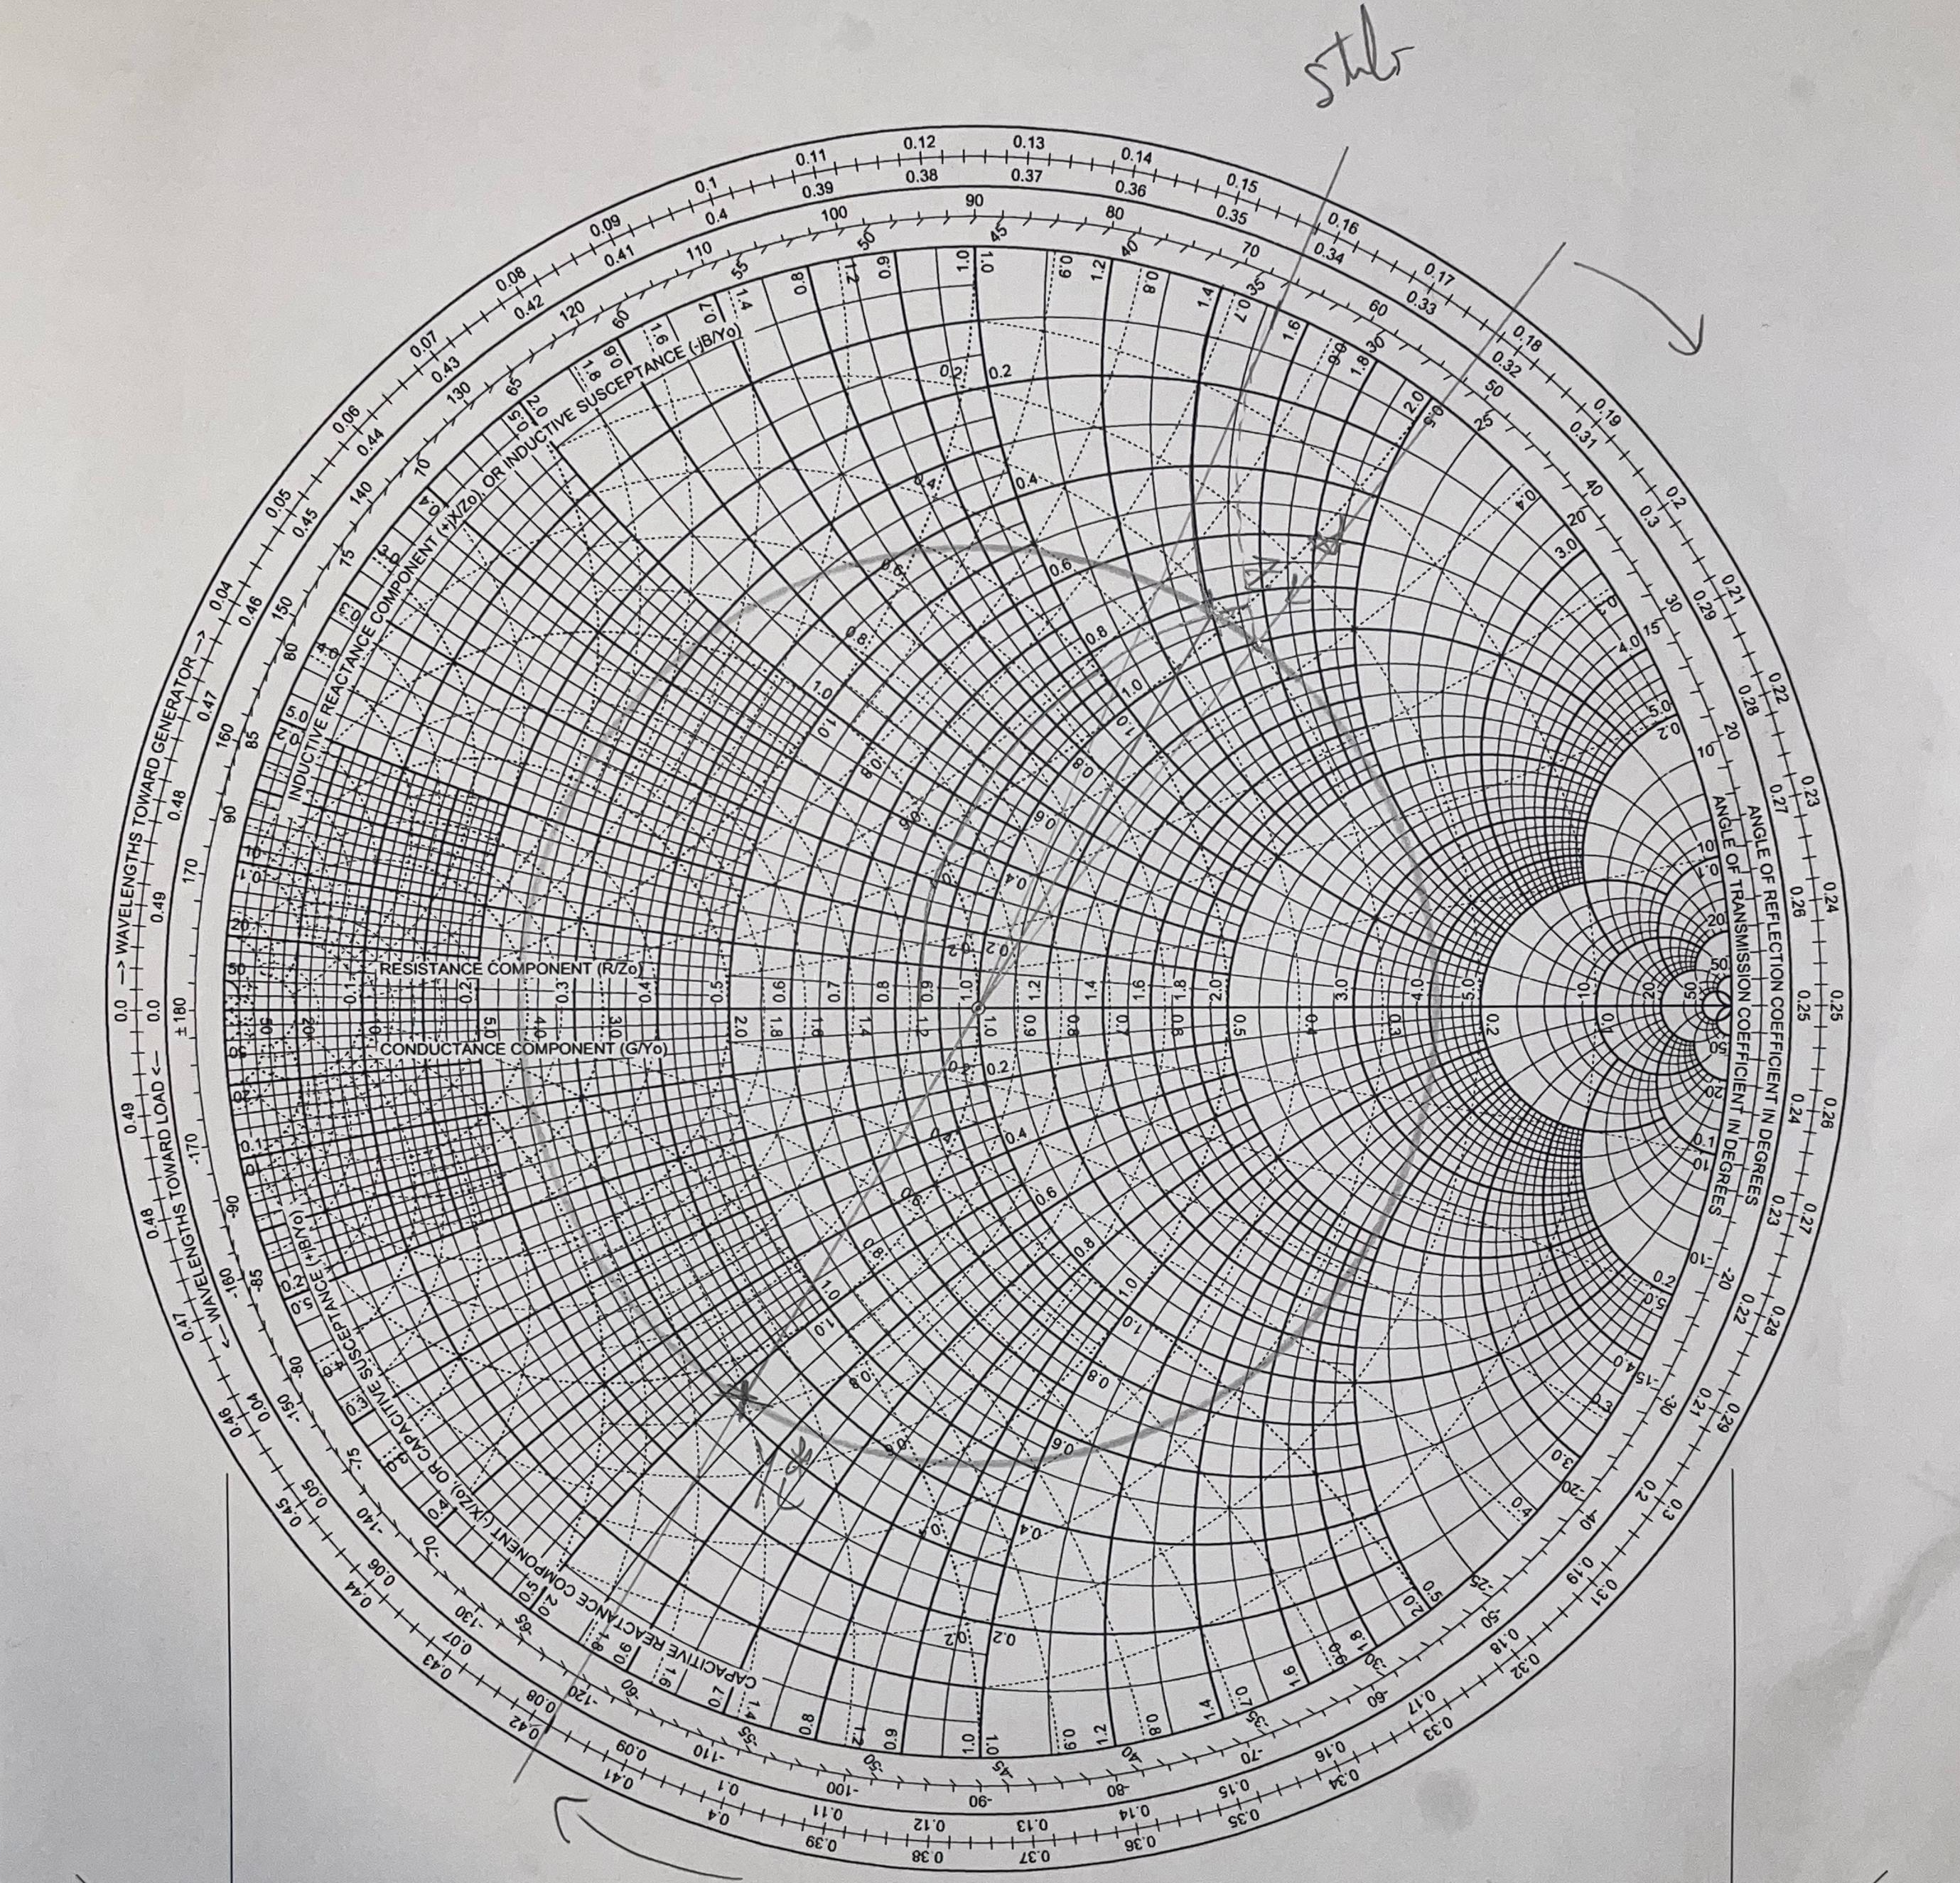
\includegraphics[width=0.5\textwidth]{Images/zl-LS-matching.png}
    \caption{Matching circuit for input with lines and stubs}
    \label{fig:zl-line-matching}
\end{figure}

The adaptation mesh for the output is done with a series line and an open circuit shunt stub.

The final circuit is shown in Figure \ref{fig:MatchingCircuit-line}, where the input and output matching networks are designed using a combination of transmission lines and stubs.

\begin{figure}[H]
    \centering
    \includegraphics[width=1\textwidth]{Images/LS_matching-circuit.png}
    \caption{Matching circuit for input and output with values}
    \label{fig:MatchingCircuit-line}
\end{figure}

%\subsection{Gain and Noise Factor}
